% Figure 1, the simple system diagram plus slider names and model copy vs real parameters. Compile standalone with: tectonic -X compile fig1_system.tex (or pdflatex)
\documentclass[border=4pt]{standalone}
\usepackage{tikz}
\usetikzlibrary{arrows.meta,fit,backgrounds,calc}
\usepackage[T1]{fontenc}
\usepackage{amsmath}
\begin{document}
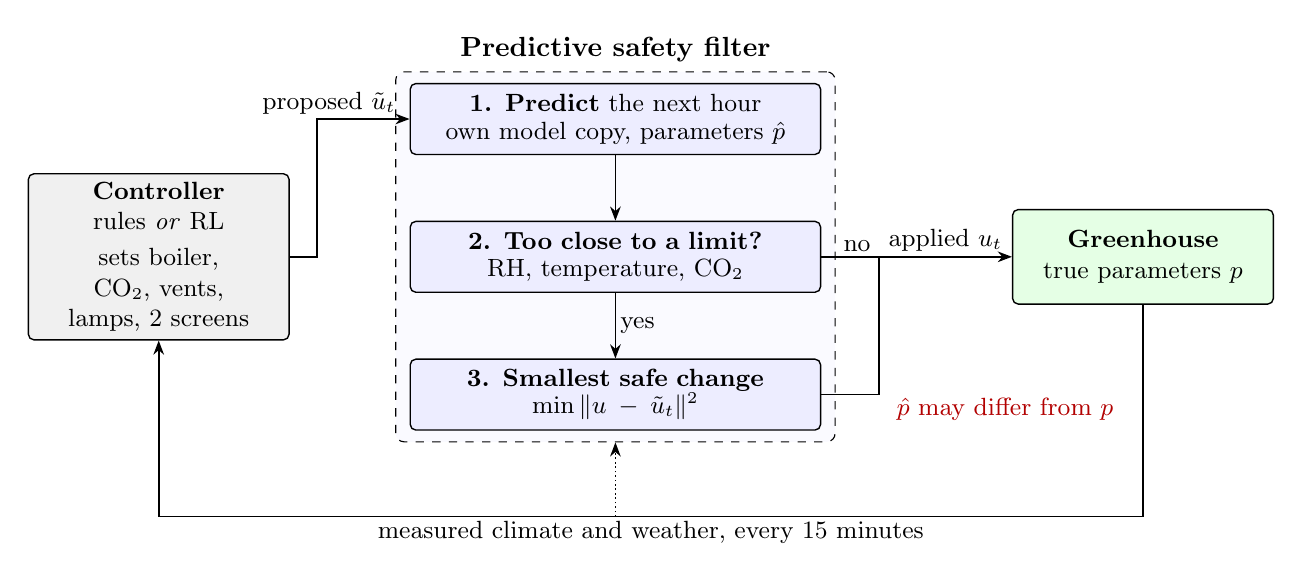
\begin{tikzpicture}[
  font=\small,
  box/.style={draw, rounded corners=2pt, align=center, inner sep=3pt, line width=0.5pt},
  ctrl/.style={box, fill=gray!12, text width=31mm, minimum height=12mm},
  plant/.style={box, fill=green!10, text width=31mm, minimum height=12mm},
  sub/.style={box, fill=blue!7, text width=50mm, minimum height=9mm},
  arr/.style={-{Stealth[length=1.8mm]}, line width=0.6pt},
  lab/.style={font=\small, align=center, inner sep=1.5pt}
]
% nodes (absolute positions, cm)
\node[ctrl]  (c)    at (-0.6, 0)      {\textbf{Controller}\\rules \emph{or} RL\\[2pt]{\small sets boiler, CO$_2$, vents,\\lamps, 2 screens}};
\node[sub]   (pred) at (5.2, 1.75) {\textbf{1. Predict} the next hour\\[-1pt]{\small own model copy, parameters $\hat p$}};
\node[sub]   (dec)  at (5.2, 0)    {\textbf{2. Too close to a limit?}\\[-1pt]{\small RH, temperature, CO$_2$}};
\node[sub]   (fix)  at (5.2, -1.75) {\textbf{3. Smallest safe change}\\[-1pt]{\small $\min\, \lVert u-\tilde{u}_t\rVert^2$}};
\begin{scope}[on background layer]
  \node[draw, dashed, rounded corners=3pt, fill=blue!2, inner xsep=5pt, inner ysep=4pt, fit=(pred)(dec)(fix)] (F) {};
\end{scope}
\node[font=\normalsize\bfseries, anchor=south] at (F.north) {Predictive safety filter};
\coordinate (m) at ($(F.east)+(0.55,0)$);
\node[plant] (g) at (11.9, 0) {\textbf{Greenhouse}\\{\small true parameters $p$}};

% forward path
\draw[arr] (c.east) -- ++(0.35,0) |- (pred.west);
\node[lab, above left] at ($(pred.west)+(-0.12,0)$) {proposed $\tilde{u}_t$};
\draw[arr] (pred) -- (dec);
\draw[arr] (dec) -- node[lab, right]{yes} (fix);
\draw[line width=0.6pt] (dec.east) -- node[lab, above, pos=0.62]{no} (m);
\draw[line width=0.6pt] (fix.east) -| (m);
\draw[arr] (m) -- node[lab, above]{applied $u_t$} (g.west);

% feedback path
\coordinate (b) at (-0.6, -3.3);
\draw[arr] (g.south) |- (b) -- (c.south);
\node[lab, anchor=north] at ($(b)!0.5!(g.south |- b)$) {measured climate and weather, every 15 minutes};
\draw[arr, densely dotted] (F.south |- b) -- (F.south);
\node[lab, text=red!70!black, anchor=north] at ($(F.south east)!0.5!(g.south)+(0.2,-0.25)$) {$\hat p$ may differ from $p$};
\end{tikzpicture}
\end{document}
